\subsection{Web-based visualization}
% why web-based? main advantages

We opted for a web-based implementation of the CLiCS visualization in JavaScript using the D3 library \cite{D3}. The main benefits of a web-based visualization are its platform independence and the fact that users can access it from any device with a browser supporting Javascript. There is no need for the installation of additional software or for maintenance of the system. In addition, links to the descriptions of the external resources can easily be included to allow users to explore the CLiCS data in more detail on demand. 

\subsection{Interactive functionalities}


% Force-directed graph; move nodes to desired position

The visualization features various interactive functionalities that are designed to enhance the exploration of the CLiCS data. The main component is a flexible force-directed graph layout that displays the concepts as nodes and the cross-linguistic polysemies as edges. The strength of the force in the edges of the graph is dependent on the number of cases that can be attested in the languages for the respective concepts that are linked through the edge. 

\begin{figure}[htbp]
\begin{center}
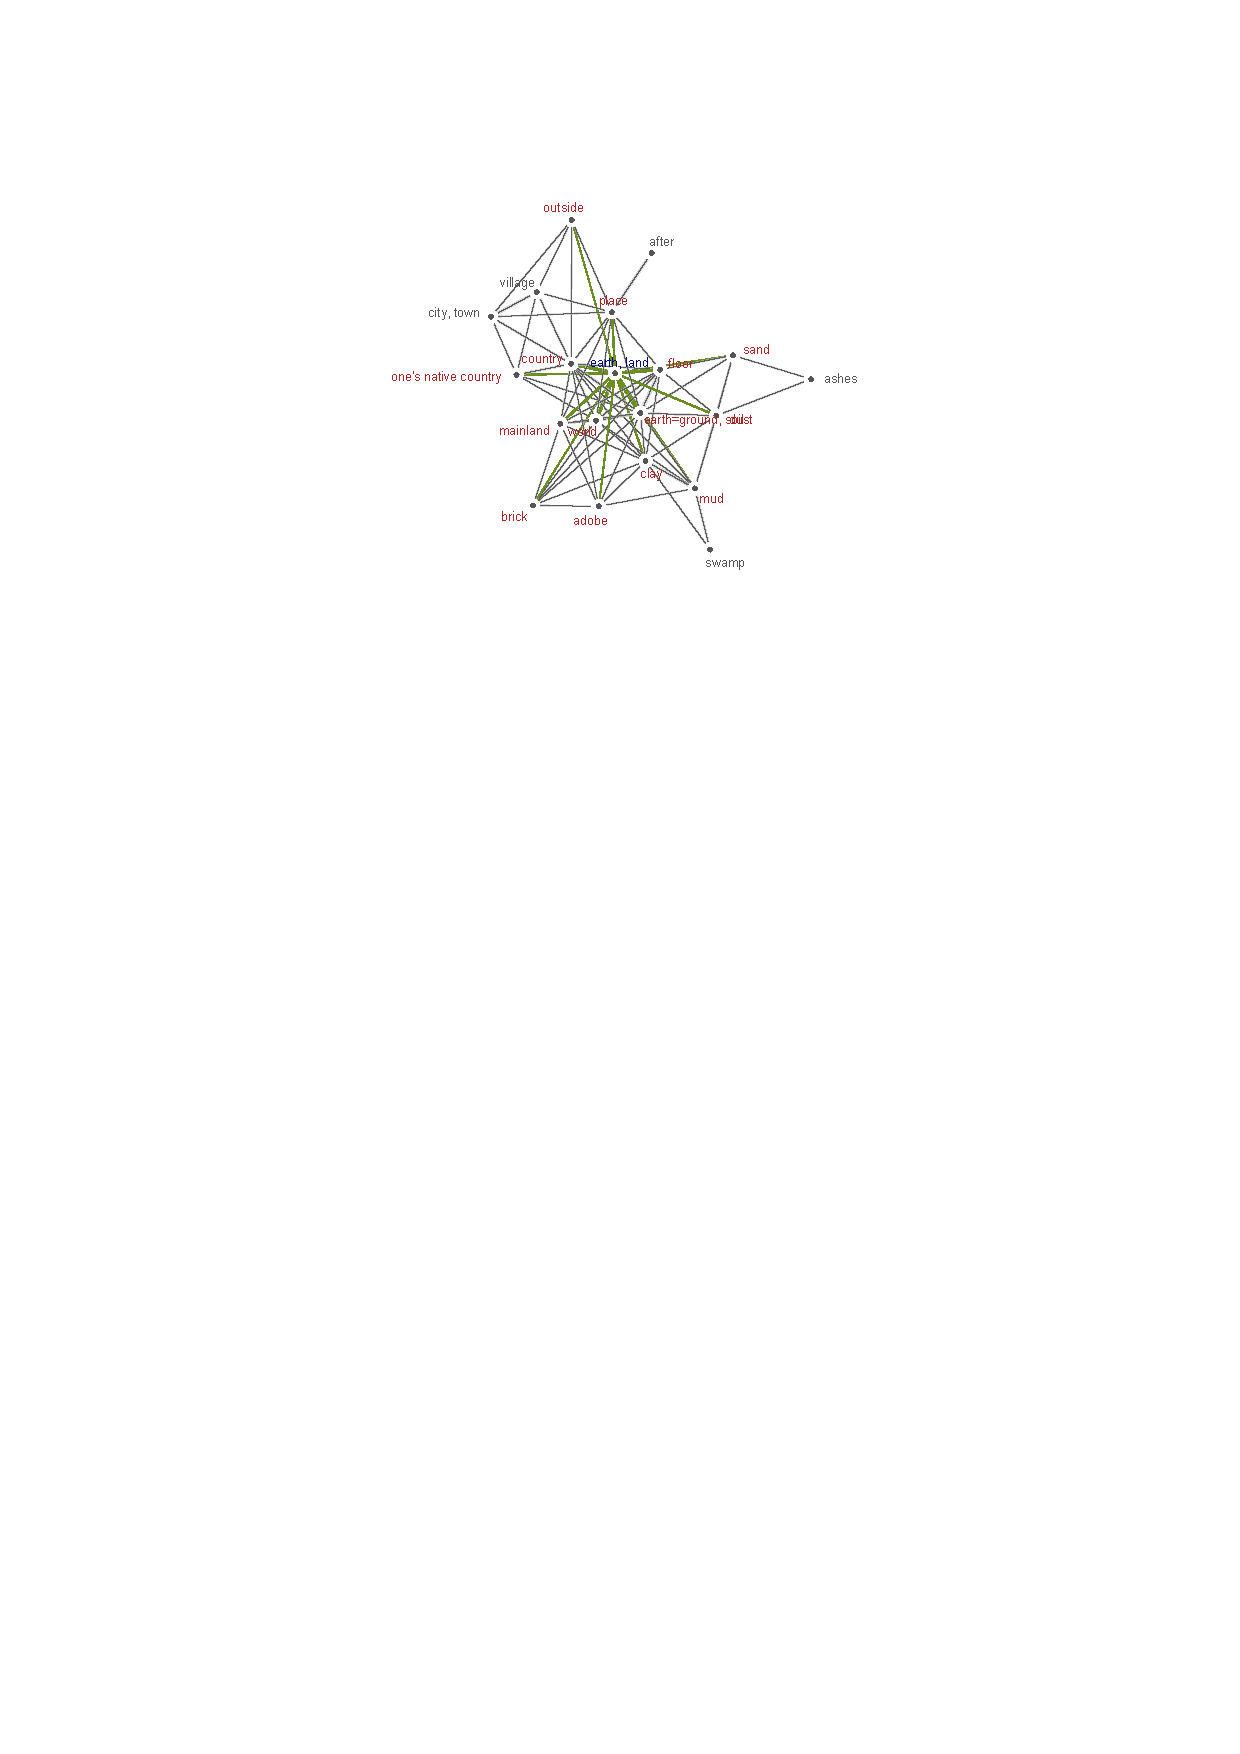
\includegraphics[width=0.48\textwidth]{img/countryconnections}
\caption{Force-directed graph with mouse-over functionalities highlighting all connected concepts}
\label{MoneySilver}
\end{center}
\end{figure}

The force-directed graph layout ensures that all concepts are neatly arranged according to their similarity as defined by the number of cross-linguistic polysemies. As a result, concepts that are highly connected are located close to each other.  To make it easier for users to explore the network that is depicted in the graph, concepts can be dragged to different positions where there is less overlap.

\begin{figure*}[htbp]
\begin{center}
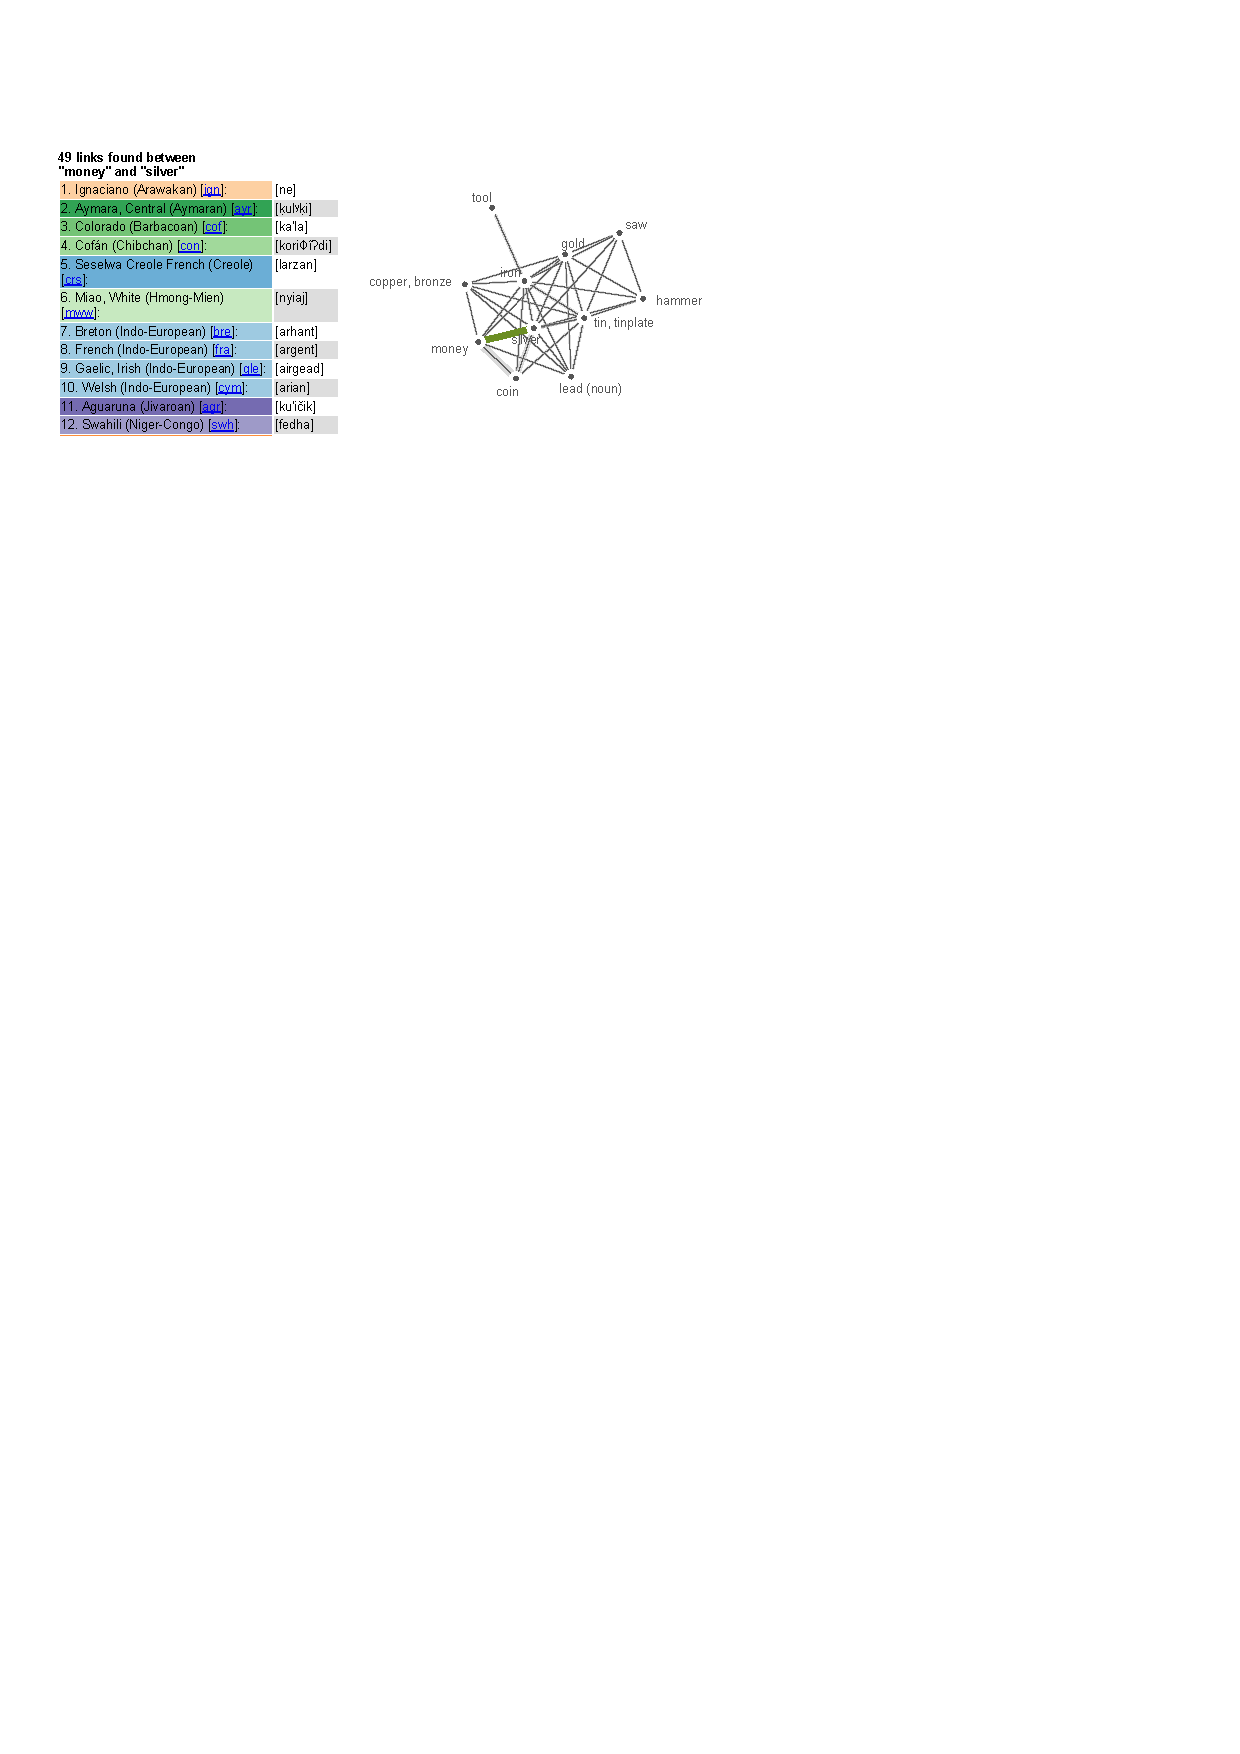
\includegraphics[width=\textwidth]{img/moneysilver.pdf}
\caption{Force-directed graph with mouse-over functionalities showing the list of words contributing to the cross-linguistic polysemies}
\label{MoneySilver}
\end{center}
\end{figure*}

\begin{figure}[htbp]
\begin{center}
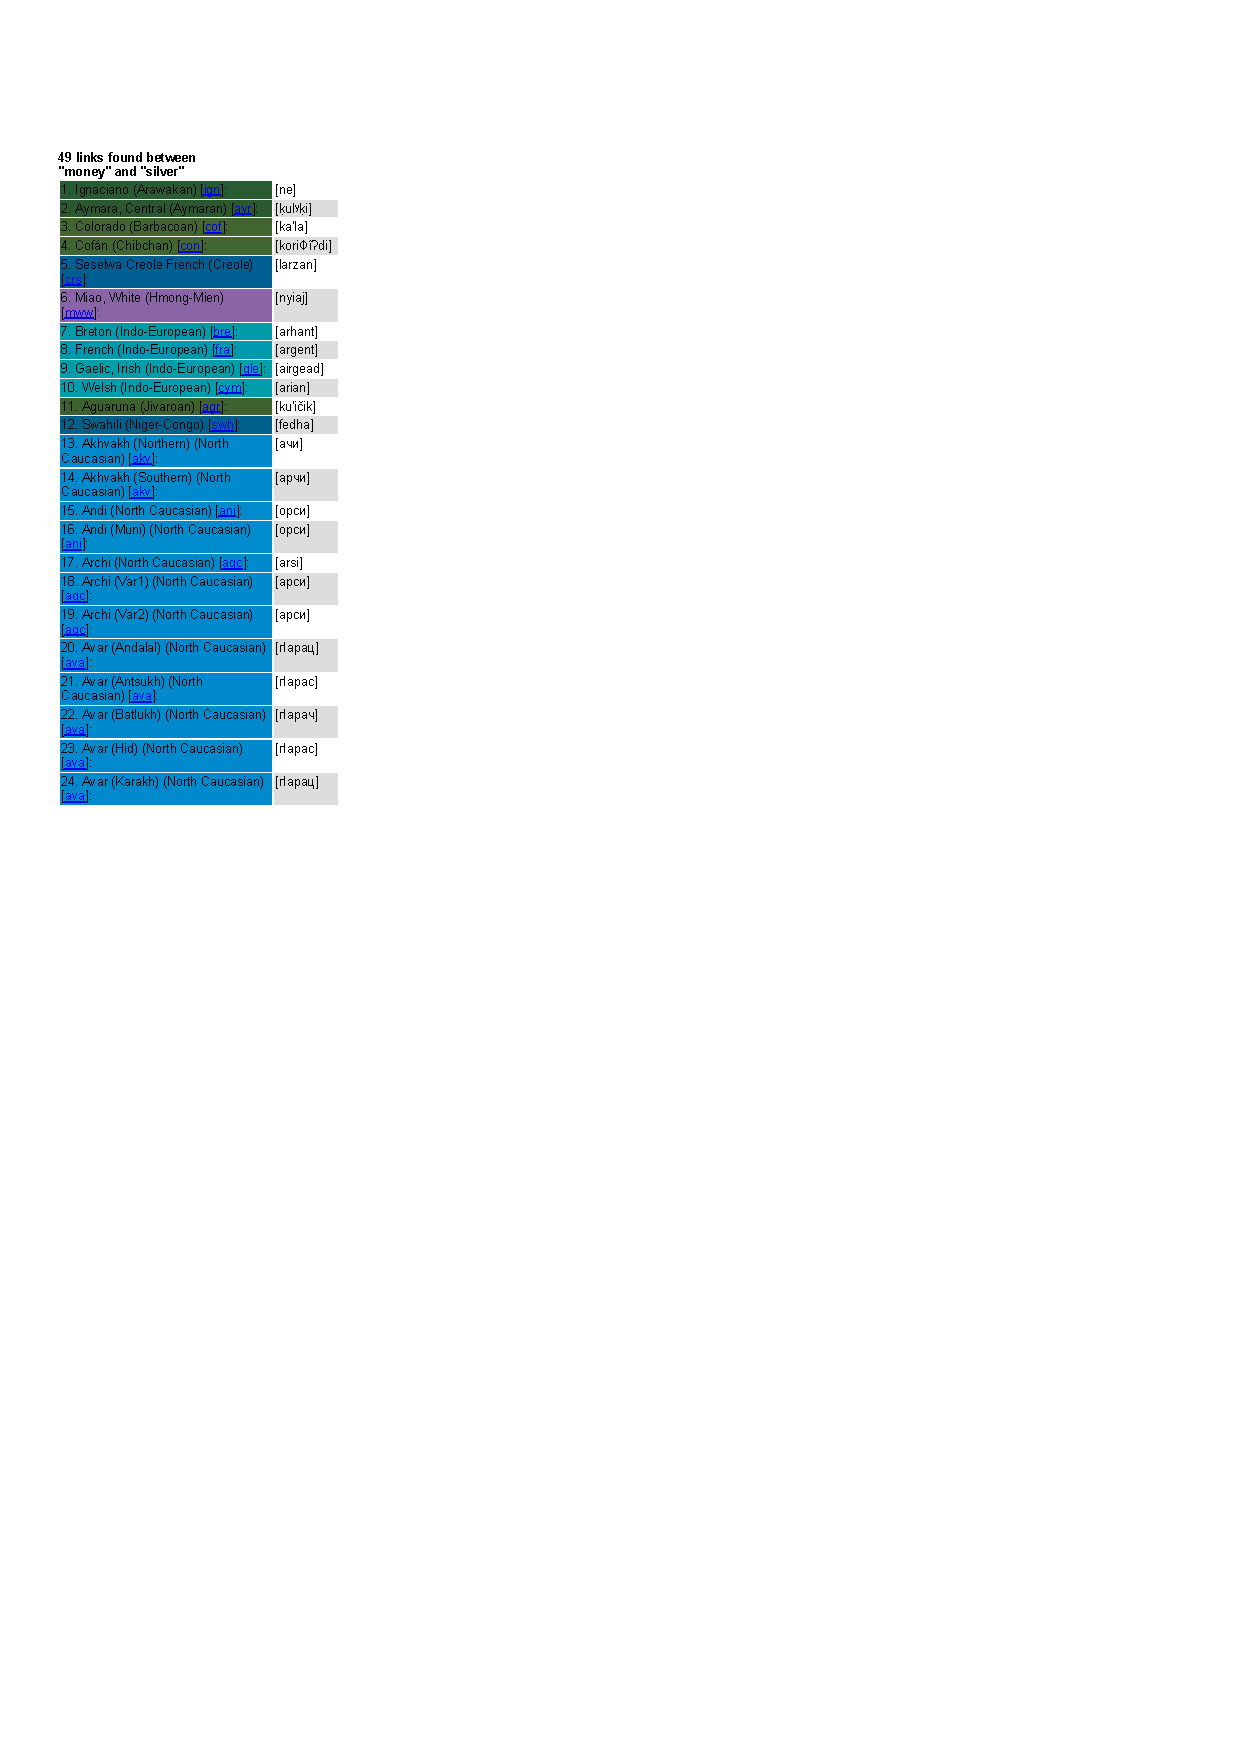
\includegraphics[width=0.238\textwidth]{img/moneysilverAreas1.pdf}
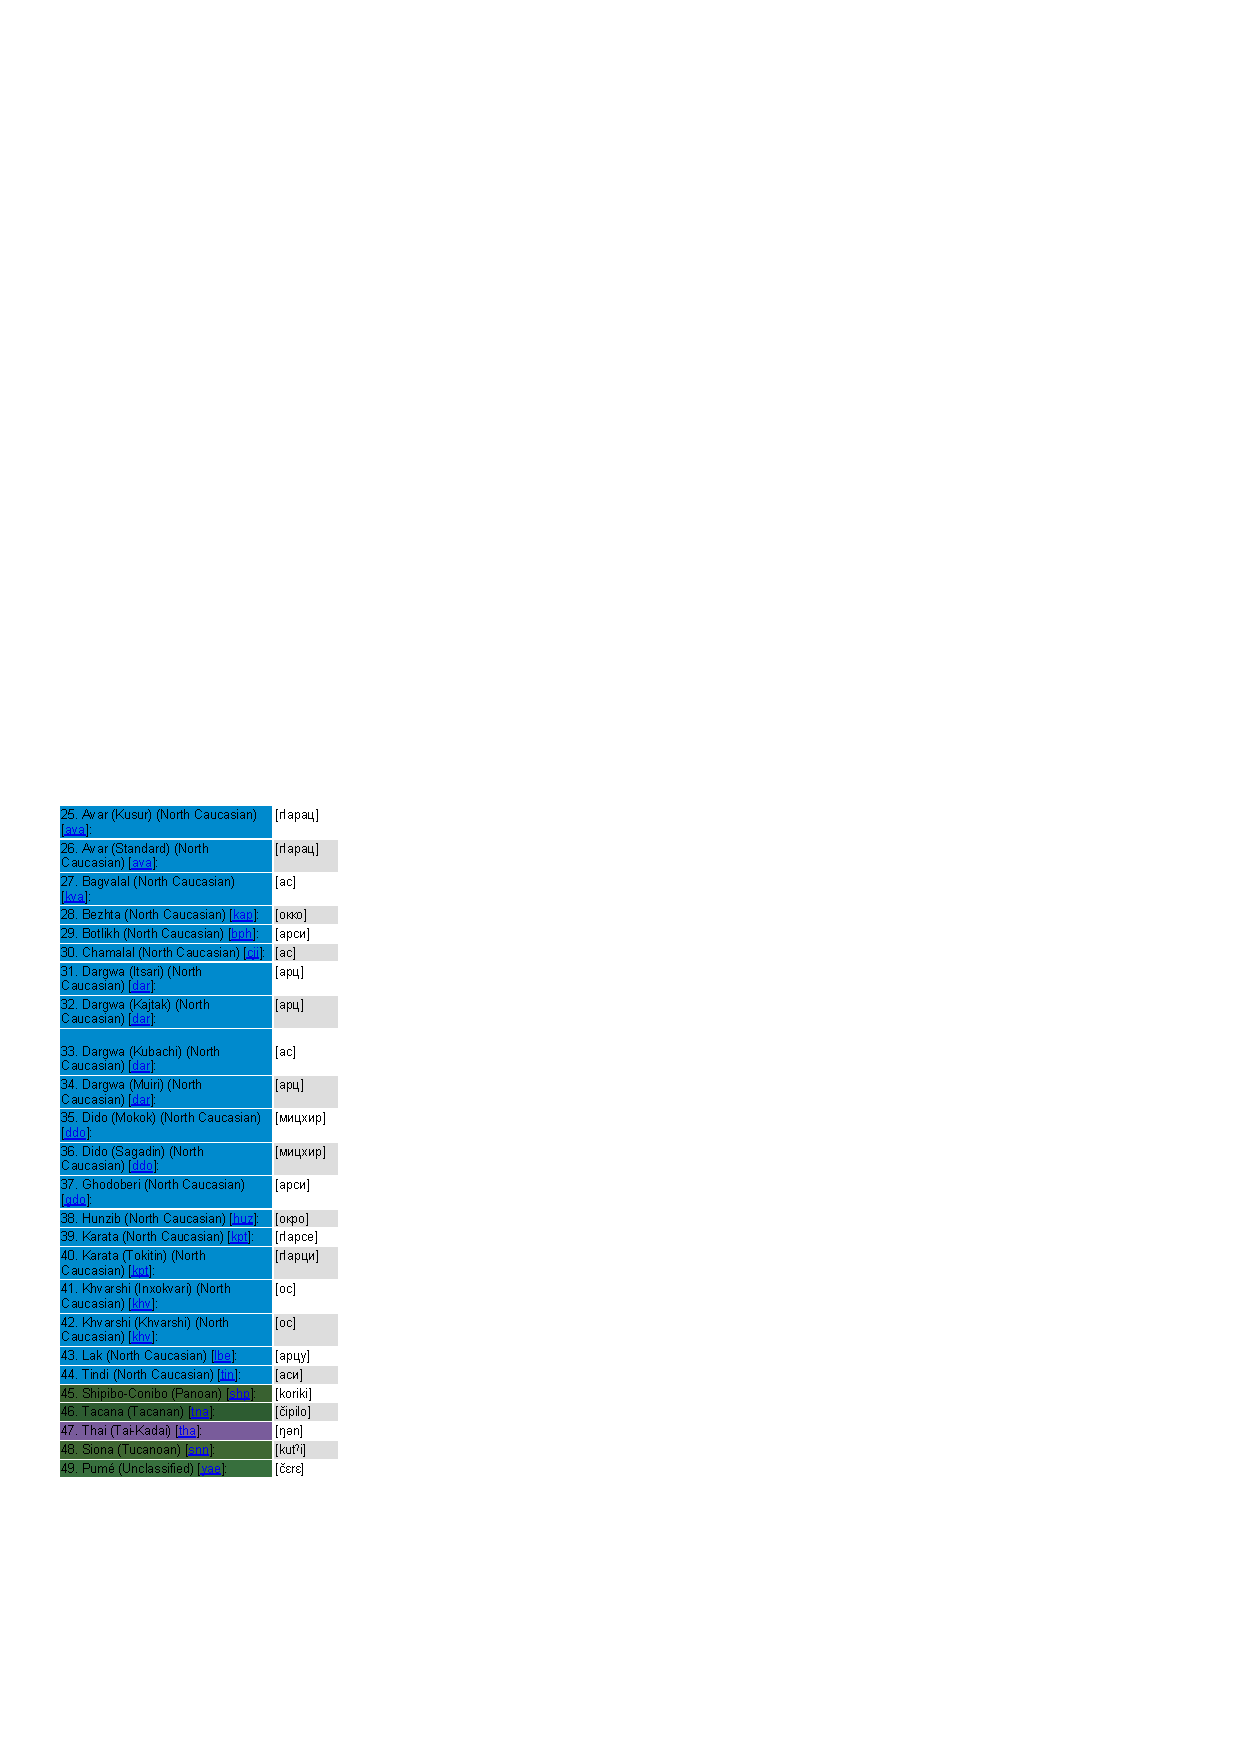
\includegraphics[width=0.238\textwidth]{img/moneysilverAreas2.pdf}
\caption{Languages and words contributing to the connections of polysemies for the concepts ``money'' and ``silver''}
\label{MoneySilverAreas}
\end{center}
\end{figure}

% mouse-over: coloring edges, show linked languages

As mentioned above, the edges of the graph represent the number of cases of cross-linguistic polysemies for the linked concepts. For a more detailed view on which languages contribute to the strength of the connections, the user can mouse over the links in the graph to see a list of  languages featuring polysemous words for the respective link. The list includes additional information on the languages such as their ISO 639-3 language code and family. Furthermore, each entry in the list provides a hyperlink to the original source from where the information is taken.  

% Color coding: families and geolocations

Each language in the list is attributed a different background color depending on its language family or location in order to allow for an at-a-glance overview for all languages in the list. The user can choose from a drop-down menu whether to include the genealogical or areal information as the background color. For the genealogical information, all language families are attributed a different color value. Languages belonging to the same language families are therefore given the same background color. Moreover, the list is sorted according to language families. In this way, the user can immediately see how many languages of  a given family contribute to the overall strength for the connection at hand. 

As to the areal information, the world map is provided with a color gradient as shown in Figure \ref{World map}. To this end, each position in the world map is attributed a color value using the L*a*b* color space. The color hue thereby indicates the position on the map in terms of the longitude (East-West) whereas the lightness of the color represents the position in terms of the latitude information (North-South). The mapping from geolocation to color values allows for an easier evaluation of areal patterns in the selected connection. In this regard, users can directly detect whether a certain cross-linguistic polysemy is restricted to a certain region of the world or constitutes a more widespread colexification pattern.

\begin{figure}[htbp]
\begin{center}
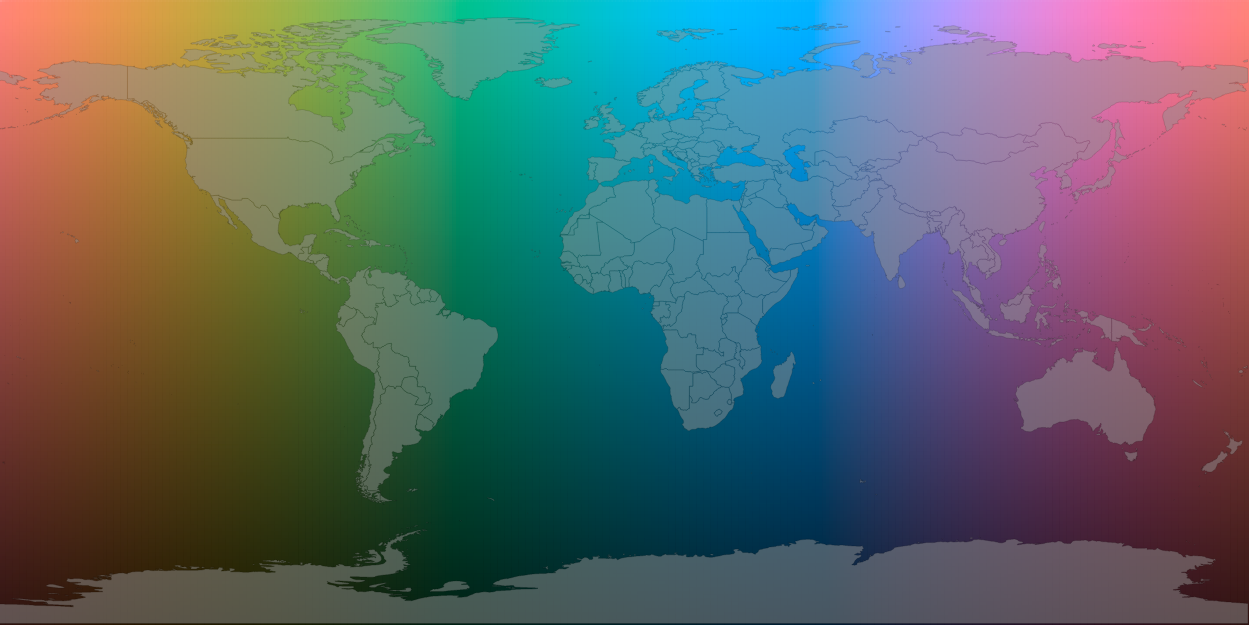
\includegraphics[width=0.48\textwidth]{img/ColorScaleWorld.png}
\caption{World map with color gradient}
\label{World map}
\end{center}
\end{figure}


% show only edges with a minimum number of links

In addition to the interactive functionalities described above, the visualization also features a variety of further components that allow for an easier exploration of the database. The graph layout is equipped with panning and zooming functionality that enables the user to navigate through the network graph. When mousing over a concept (node) in the graph all connected links and concepts are highlighted
in order to provide a better overview of the connectivity of certain concepts. The control panel of the visualization also includes a slider button that allows the user to show only those edges in the graph with a minimum number of cross-linguistic polysemies. 

% zooming and panning



\subsection{Implementation}
% description of D3 and the implementation

The visualization is implemented in JavaScript using the D3 library \cite{D3}. The force-directed graph is  generated with the \texttt{force()} function from the \texttt{d3.layout} module. The layout implementation uses position Verlet integration for simple constraints.\footnote{See \url{https://github.com/mbostock/d3/wiki/Force-Layout} for a description of the implementation.}

The color values are computed from the two-dimensional geographical coordinates that are given as an input. The latitude [-90;90] and longitude [-180;180] values are thereby normalized between [0;1] and serve as the input for the function \texttt{cl2pix}.\footnote{The code was taken from \url{http://davidad.net/colorviz/} and translated into JavaScript.}

\begin{verbatim}
function cl2pix(c,l){
   		var TAU = 6.2831853 
   		var L = l*0.61 + 0.09; 
   		var angle = TAU/6.0 - c*TAU;   
   		var r = l*0.311 + 0.125 
   		var a = Math.sin(angle)*r;
   		var b = Math.cos(angle)*r;
   		return [L,a,b];
 };
\end{verbatim}

The actual HTML color code is generated with the function \texttt{d3.lab} from the D3 library, which takes as input the three values for \texttt{[L,a,b]}.

\subsection{Case study}

In order to illustrate the usefulness of the visualization for the purposes of exploring the database, consider the graph in Figure \ref{MoneySilver}. Among other things, it contains the connection between the concepts ``money'' and ``silver''. A subset of the languages and words contributing to this connection are shown on the left where the background color represents the language families. For instance, French contributes to the cross-linguistic polysemy because both concepts are realized by the same word (viz. \textit{argent}) in that language. When looking at the areal distribution of the languages, a clear pattern emerges at a glance (see Figure \ref{MoneySilverAreas}). Most of the languages contributing to the polysemy are from two major regions: Caucasus (marked in blue) and South America (marked in green).  


